% Chapter Template

\chapter{Results} % Main chapter title

\label{Chapter5} % Change X to a consecutive number; for referencing this chapter elsewhere, use \ref{ChapterX}

%----------------------------------------------------------------------------------------
%	SECTION 1
%----------------------------------------------------------------------------------------

\section{Data insights on beneficiaries}
\label{BSratio}

\subsection{Liquidity}

In figure \ref{fig:Ratios} the calculated ratios for all companies of the dataset are shown with boxplots for the years 2018-202. With the median, shown as the middle line in the box, the first and the third quartile, boxplots allow a simple comparison between the years that is not sensitive for outliers. The three observed liquidity ratios show an increase in liquidity in 2020 and 2021 compared to the pre pandemic years, indicating that companies were holding relatively more cash at the year-end since the pandemic. 
Overall, the observations are in line with a study conducted by the German Federal Bank that also reported an increase in the average cash ratio for the whole population German companies in 2020 as well as in 2021 \parencite{deutsche_bundesbank_jahresabschlussstatistik_2022}. For example, for SME corporations the study reported a change in the cash ratio from 0.104 (2019) to 0.110 (2020). For the current ratio and quick ratio, the same trend was reported. Further support for an increase in the quick ratio comes from another study by \parencite{bley_mittelstand_2022}. Although the exact ratios are varying between studies, there is strong support for the general trend of increasing liquidity in 2020 and 2021.
What also can be seen in figure \ref{fig:Ratios} is that the whiskers of the boxplots are longer in the pandemic years, showing the heterogeneity of liquidity levels for firms. Considering that the ratios only reflect that status of the cutoff date, this can also be an indicator that the liquidity levels of firms are more volatile than before the pandemic which could be caused by forecasting difficulties in the liquidity planning during the pandemic. 


\subsection{Solvency}

Solvency ratios are showing a less clear trend after the COVID-19 pandemic. Although minimal, the opposite trends in the equity ratio and debt-to-asset-ratio are as expected. The only visible change happened in 2020, while in 2021 the ratios are very similar to 2018 and 2019. The change in the debt-to-asset ratio is amplified in the debt-to-equity ratio, as expected. Survey Data from the KFW found an Equity Ratio of 0.318 in 2019, a decrease to 0.301 in 2020 and a recovery to 0.314 in 2021 \parencite{kfw_kfw-mittelstandspanel_2022}. For very small companies with less than 10 employees, the drop in 2020 was stronger, and the recovery in 2021 was above pre-pandemic levels. On the other hand, the survey reported
that larger companies did not have a recovery after the first crisis year and decreased their Equity Ratio in 2021 on average further. 
This could indicate that the recovery of the indebtedness of beneficiaries in 2021 might have been driven by smaller companies. Similar observations were reported by the German Federal Bank were the debt-to-asset-ratio for SME corporations decreased in 2020 \parencite{deutsche_bundesbank_jahresabschlussstatistik_2022}.



\begin{figure}
\centering
\makebox[\textwidth][c]{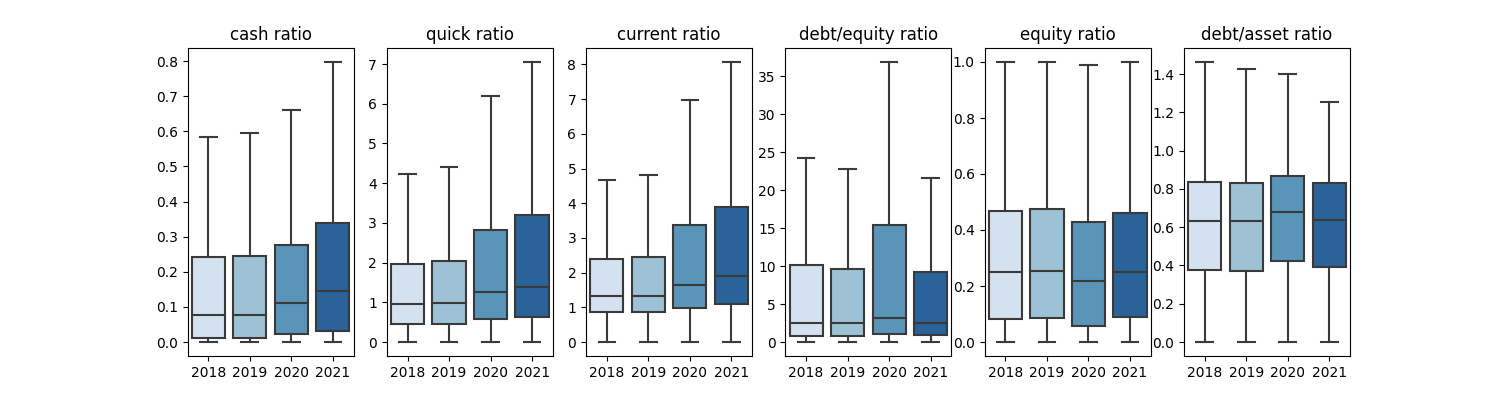
\includegraphics[width=1.3\columnwidth]{Figures/chart_ratios}}%

\decoRule
\caption[Balance sheet ratios]{Boxplots with balance sheet ratios from the obained dataset. Extreme outliers above the maximum values are not shown.}
\label{fig:Ratios}
\end{figure}






\subsection{Insolvencies of beneficiaries}


In total 953 insolvent firms were identified representing a share of 0.92 \% of all beneficiaries of pandemic aid from transparency database, as shown in table \ref{tab:InsBySize}. A further breakdown reveals that the share of SMEs is significantly lower than their larger counterparts. Due to the fact that the transparency database only provides very few beneficiaries with aid payments below 100.000 EUR, smaller companies with aid below the threshold are not well represented. Therefore, the numbers only give an indication.

\begin{table}
    \caption{Share of insolvent aid  beneficiaries by size}
    \label{tab:InsBySize}
    \centering
    \def\arraystretch{1.2}
    \centering
    \begin{tabular}{lrrl}
\toprule
           size &  aid beneficiaries &  insolvent & share \\
\midrule
           SMEs &              78077 &        526 & 0.67\% \\
Large companies &              25259 &        427 & 1.69\% \\
          Total &             103336 &        953 & 0.92\% \\
\bottomrule
\end{tabular}
}

    \small  Notes: 

\end{table}

In the next step the industries of insolvent beneficiaries were analyzed. The results for the most represented industries are presented in table \ref{tab:InsByIndustry_short}. A more comprehensive table with more industries is in Appendix \ref{AppendixB}. The findings show that food and beverage service activities is the industry with most beneficiaries, but only has a share 0.58 \% of insolvencies that well below the average. 

Similarly, the accommodation sectors is highly represented. With only 24 insolvencies out of 9.885 recipients is has the lowest share amongst the most represented industries. On the higher end are specialized construction activities with a share of 1.66 \%. The closely related construction building sector has an even higher share with 2.97 \%, but is less represented and therefore only shown in the appendix. Partially, even higher shares are present in the data, but only in underrepresented industries. 

\begin{table}
    \caption{Share of insolvent aid  beneficiaries by industry}
    \label{tab:InsByIndustry_short}
    \centering
    \def\arraystretch{1}
    \centering
    \begin{tabular}{lrrl}
\toprule
                                industry &  beneficiaries &  insolvent & share \\
\midrule
    Food and beverage service activities &          15173 &         88 & 0.58\% \\
Retail trade, except of motor vehicles a &           8810 &         84 & 0.95\% \\
     Specialised construction activities &           4103 &         68 & 1.66\% \\
Wholesale trade, except of motor vehicle &           5396 &         56 & 1.04\% \\
Manufacture of fabricated metal products &           3105 &         40 & 1.29\% \\
Office administrative, office support an &           3040 &         28 & 0.92\% \\
Sports activities and amusement and recr &           5232 &         27 & 0.52\% \\
                           Accommodation &           9885 &         24 & 0.24\% \\
Wholesale and retail trade and repair of &           3525 &         17 & 0.48\% \\
\bottomrule
\end{tabular}
}

    \small  Notes: Tables shows industries with more than 3000 beneficiaries and is sorted by insolvencies.

\end{table}




\subsection{Ratios of insolvencies}

Next, the ratios of insolvent beneficiaries are analyzed and compared to the other beneficiaries. For the comparison the cash ratio and the debt-to-asset-ratio are chosen to analyze the liquidity and solvency. Figure \ref{fig:RatiosInsolvency} shows the already for section \ref{BSratio} used boxplot, but grouped into solvent (light blue) and insolvent by the spring 2023 (darker blue). For the liquidity ratio a clear discrepancy can be observe throughout all periods. The group of companies that later got insolvent has already before 2020 significantly less liquidity than the other group. However, in 2020 and 2021 their cash ratio is also increasing, like the solvent group.
The debt-to-asset-ratio comparison also shows a clear gap between both groups. The companies which are later becoming insolvent have a higher leverage before and after the start of the pandemic. 

\begin{figure}
    \centering
    \makebox[\textwidth][c]{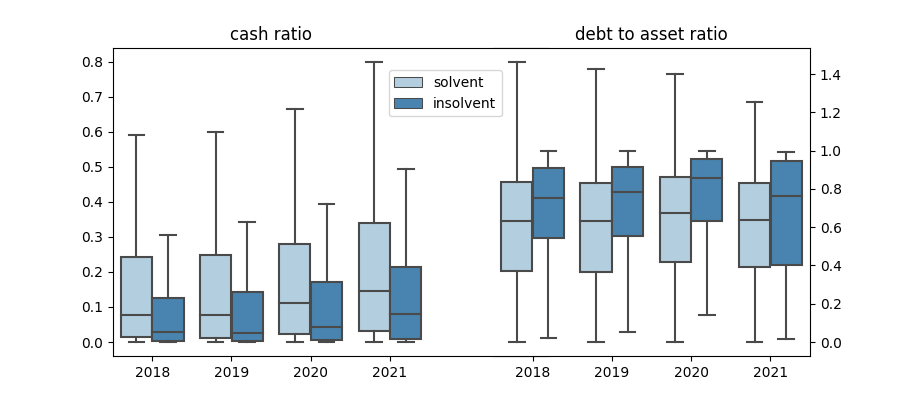
\includegraphics[width=1.2\columnwidth]{Figures/chart_ratios_insolvence}}%
    
    \decoRule
    \caption[Balance sheet ratios]{Boxplot with balance sheet ratios from the obained dataset.}
    \label{fig:RatiosInsolvency}
\end{figure}





%----------------------------------------------------------------------------------------
%	SECTION 2
%----------------------------------------------------------------------------------------

\section{The effect of government support}



\subsection{The average effect on firm liquidity}



The interaction terms from the difference-in-differences regressions are shown in table \ref{tab:DiDresults}. 
The coefficients for the aid and post coefficients are reported in Appendix \ref{AppendixA}. In the first-row cash ratio coefficients are reported for grants and loans. In the 2020 column the effect for grants is the only cash ratio coefficient that is not statistically significant. 

In 2021 the coefficient for grants on the cash ratio was estimated to be 7.68 \% indicating a strong causal effect. The average treatment effect for firms that got aid through loans is positive in 2020 and 2021, but less strong than grants. Also, the effect in 2021 is less strong compared to 2021.

The quick ratio and the current ratio only have statistical significance for loans. At a significance level of 1 \% only the quick ratio and the current ratio coefficient for 2020 are significant. The treatment effects with 10.85 \% and 12.71 \% are even stronger than for the cash ratio. The effects for the current ratio are even larger, reflecting the proportionality between the ratios. Overall, the results show strong effects of loans on the observed liquidity ratios. For grants an even stronger effect was observed in 2021, but only for the cash ratio, not for the more conservative ratios. However, this could be caused by the alternative calculation of the quick and current ratio that was used for part of the companies. 

In summary both aid measures have a significant effect on the cash ratio indicating a liquidity boost. The measured increase in liquidity through loans indicates that they were not used for refinancing existing debt, but served as liquidity injection as intended by the policy makers.

\subsection{The average effect on solvency of firms}

In the row for the debt-to-equity ratio strongly positive coefficients were observed for loans in 2020 and 2021. Since the debt-to-equity ratio reflects a firm's leverage it is plausible that loans have a causal effect on debt. Regarding the equity ratio in following row a negative effect of loans was estimated for 2020 and 2021. For grants, which aren't affecting a firm's debt, no statistically significant effect was observable and thus indicating that grants didn't support the equity of firms. Further support for the increase in leverage through loans comes from the debt-to-asset ratio coefficients. The effects for loans are strong in 2020 and 2021 with 7.15 \% and 5.26 \%. 
For grants the causal effect is 4,12 \% in 2020 and reversing in 2021 to - 3.02 \%. The positive effect in 2020 is in line with missing effect on the equity ratio. The negative coefficient in 2021 on the other hand, indicates that grants helped firm's to reduce leverage by slightly.

In summary, the increase in leverage from loans is measurable as expected. However, the estimates doesn`t support the expectation that grants protect the equity of firms. The positive effect of grants on the debt-to-asset ratio and the missing effect on the cash ratio in 2020 suggest that the grants were not sufficient to prevent liquidity short falls and therefore companies had to rely on debt from other sources for additional liquidity. The reversal of the effect on the debt-to-asset ratio and the effect on the cash ratio in 2021 suggest that grants only became effective in providing sufficient liquidity and reducing leverage in 2021. However, this could be related to the fact that only relatively little grants were provided in 2020.

\begin{table}
    \caption{Government aid impact on ratios}
    \label{tab:DiDresults}
    \centering
    \def\arraystretch{1.2}
    \centering
    \begin{tabular}{llrr}
\toprule
                     & \textbf{year} &                                    2020 &                                    2021 \\
{} & \textbf{instrument} &                                         &                                         \\
\midrule
\multirow{2}{*}{\textbf{cash ratio}} & \textbf{grant} &  -0.0089\space\space\space\space(0.270) &                  0.0768***\space(0.000) \\
                     & \textbf{loan} &                  0.0527***\space(0.000) &                  0.0351***\space(0.000) \\
\cline{1-4}
\multirow{2}{*}{\textbf{quick ratio}} & \textbf{grant} &  -0.0937\space\space\space\space(0.221) &   0.0913\space\space\space\space(0.478) \\
                     & \textbf{loan} &                  0.1085***\space(0.000) &   0.0929\space\space\space\space(0.252) \\
\cline{1-4}
\multirow{2}{*}{\textbf{current ratio}} & \textbf{grant} &  -0.0825\space\space\space\space(0.330) &   0.0476\space\space\space\space(0.736) \\
                     & \textbf{loan} &                  0.1271***\space(0.000) &        0.1828*\space\space\space(0.064) \\
\cline{1-4}
\multirow{2}{*}{\textbf{debt to equity ratio}} & \textbf{grant} &        0.2478*\space\space\space(0.089) &  -0.1592\space\space\space\space(0.185) \\
                     & \textbf{loan} &                  0.7306***\space(0.000) &             0.5043**\space\space(0.016) \\
\cline{1-4}
\multirow{2}{*}{\textbf{equity ratio}} & \textbf{grant} &  -0.0112\space\space\space\space(0.371) &   0.0108\space\space\space\space(0.465) \\
                     & \textbf{loan} &                 -0.0486***\space(0.000) &                  -0.037***\space(0.004) \\
\cline{1-4}
\multirow{2}{*}{\textbf{debt to assest ratio}} & \textbf{grant} &                  0.0412***\space(0.006) &       -0.0302*\space\space\space(0.079) \\
                     & \textbf{loan} &                  0.0715***\space(0.000) &                  0.0526***\space(0.002) \\
\bottomrule
\end{tabular}
}

    \small  Notes: Standard errors in parentheses, *** p<0.01, ** p<0.05, * p<0.1

\end{table}




\subsection{Aid effect on companies that later become insolvent}

The group of future insolvent companies was used for a another difference in differences experiment to estimate the treatment effect of aid on the subgroup. Results are shown in table \ref{tab:DiDresultsInsolvent}. Two coefficients with statistical significance were identified, both in 2020 and for loans. First, the treatment effect of aid was 0.0427 on the cash ratio. The effect is weaker than the 0.527 that was estimated on the complete data set. This can be understood that these companies absorbed the liquidity from loans quicker due to a greater need of liquidity. The other slightly significant coefficient indicates a positive effect on the debt-to-asset-ratio of 0.0882 which is also higher than the overall effect observed from all companies.  This shows that despite the loan based aid measures the later insolvent companies had a greater chance of indebtedness, than other companies.
The higher debt-to-asset-ratio could also be an indication of that these companies used debt from other sources. In any case, the, additional indebtedness increased the risk for insolvency.



        

\begin{table}
    \caption{Government aid impact on ratios}
    \label{tab:DiDresultsInsolvent}
    \centering
    \def\arraystretch{1.2}
    \centering
    \begin{tabular}{llrr}
\toprule
                     & \textbf{year} &                                    2020 &                                    2021 \\
{} & \textbf{instrument} &                                         &                                         \\
\midrule
\multirow{2}{*}{\textbf{cash ratio}} & \textbf{grant} &   -0.038\space\space\space\space(0.605) &   0.1469\space\space\space\space(0.337) \\
                     & \textbf{loan} &             0.0427**\space\space(0.046) &  -0.1302\space\space\space\space(0.394) \\
\cline{1-4}
\multirow{2}{*}{\textbf{quick ratio}} & \textbf{grant} &   0.2732\space\space\space\space(0.645) &   0.4531\space\space\space\space(0.598) \\
                     & \textbf{loan} &   0.1349\space\space\space\space(0.493) &   0.2365\space\space\space\space(0.728) \\
\cline{1-4}
\multirow{2}{*}{\textbf{current ratio}} & \textbf{grant} &   0.2117\space\space\space\space(0.759) &   0.3419\space\space\space\space(0.666) \\
                     & \textbf{loan} &   0.0444\space\space\space\space(0.848) &  -0.0784\space\space\space\space(0.930) \\
\cline{1-4}
\multirow{2}{*}{\textbf{debt to equity ratio}} & \textbf{grant} &  -3.9105\space\space\space\space(0.867) &   1.0318\space\space\space\space(0.588) \\
                     & \textbf{loan} &   2.0475\space\space\space\space(0.262) &   6.8704\space\space\space\space(0.663) \\
\cline{1-4}
\multirow{2}{*}{\textbf{equity ratio}} & \textbf{grant} &   0.0889\space\space\space\space(0.588) &  -0.1444\space\space\space\space(0.405) \\
                     & \textbf{loan} &  -0.0338\space\space\space\space(0.381) &  -0.2779\space\space\space\space(0.467) \\
\cline{1-4}
\multirow{2}{*}{\textbf{debt to assest ratio}} & \textbf{grant} &   0.0797\space\space\space\space(0.650) &  -0.0763\space\space\space\space(0.728) \\
                     & \textbf{loan} &        0.0892*\space\space\space(0.080) &   0.1806\space\space\space\space(0.580) \\
\bottomrule
\end{tabular}
}

    \small  Notes: Standard errors in parentheses, *** p<0.01, ** p<0.05, * p<0.1

\end{table}
    



%----------------------------------------------------------------------------------------
%	SECTION 3
%----------------------------------------------------------------------------------------

\section{Causal Curve}


 
    